\section{AdaBoost}
\subsection{Adaptives Lernen}
Ein Großteil der Boosting-Algorithmen benutzt das Prinzip des sequenziellen adaptiven Lernens. Das heißt, dass man die Lerner sequentiell, also nacheinander, so trainiert, dass jeder Lerner versucht adaptiv die Fehler des vorherigen Lerners auszubessern.
\newline
Der Vertreter dieser Methode ist der AdaBoost-Algorithmus, dessen Name sich von 'Adaptive Boosting' ableitet.
\subsubsection{Gewichtete Daten}
Um einen Lerner in einem Boosting-Algorithmus zu entwickeln, wird der Lernalgorithmus zunächst auf dem ursprünglichen Datensatz angewendet. Nach dieser ersten Runde bewertet der Algorithmus die Klassifikationsergebnisse, um festzustellen, welche Datenpunkte richtig und welche falsch klassifiziert wurden. Die falsch klassifizierten Datenpunkte erhalten dann ein höheres Gewicht, was ihre Bedeutung im Datensatz für den nächsten Schritt erhöht. Im Gegenzug werden die Gewichte der korrekt klassifizierten Datenpunkte verringert.
\newline
In der darauffolgenden Iteration wird der Lernalgorithmus erneut angewendet, diesmal aber auf den Datensatz, dessen Gewichte gerade angepasst wurden. Dadurch wird der Lernalgorithmus versuchen sich besonders auf die vom ersten Lerner falsch klassifizierten Daten zu konzentrieren. Nach dem Training des zweiten Lerners erfolgt eine weitere Anpassung der Gewichte nach den gleichen Regeln.
\newline
Dieser Prozess wird fortgesetzt, wobei jeder nachfolgende Lerner, darauf abzielt, die Fehler seiner Vorgänger zu korrigieren (siehe \autoref{fig:Geron2017Abb7-7}).

\begin{figure}[h]
    \centering
    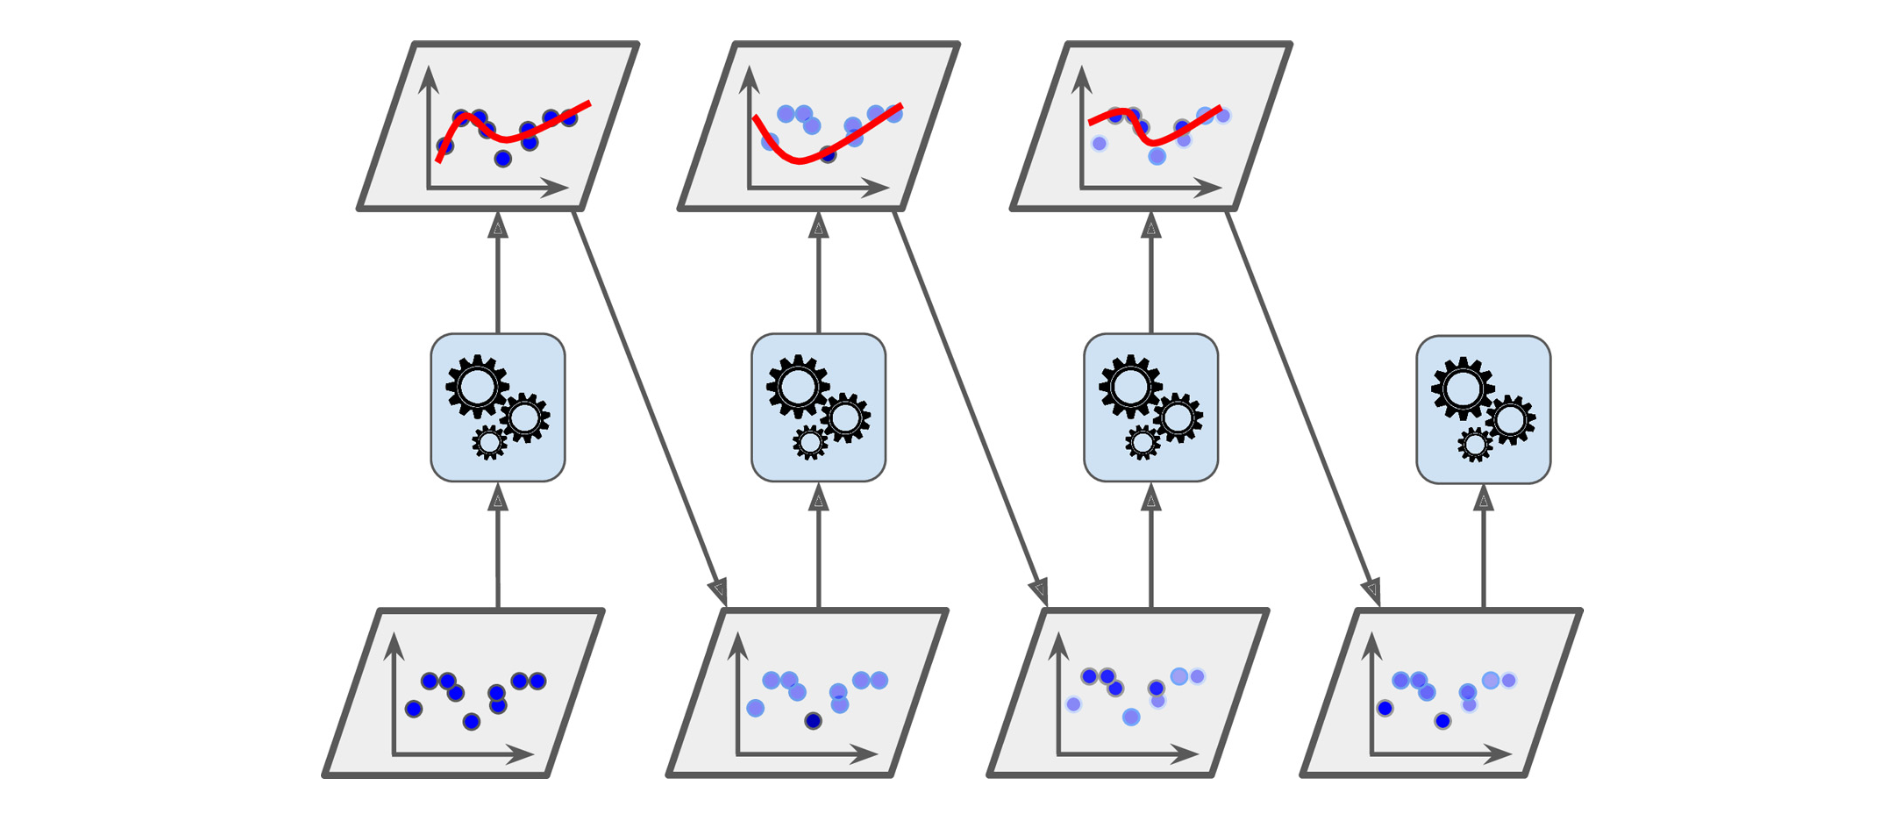
\includegraphics[width=\linewidth]{Images/Geron2017Abb7-7.png}
    \caption{Sequentielles Training mit aktualisierten Gewichten der Datenpunkte bei AdaBoost nach \textcite[Abbildung 7-7][S.~192]{Geron2018}}
    \label{fig:Geron2017Abb7-7}
\end{figure}

\subsection{Algorithmus-Struktur und Funktionsweise}
Der AdaBoost-Algorithmus (siehe Algorithmus~\ref{fig:adaboost}) ist in mehrere Schritte unterteilt, welche im folgenden genau erklärt werden:

\paragraph{Schritt 1: Initialisierung (Zeile 2)}
Hier werden die Gewichte \( D_1(i) \) initial gleich verteilt. Das heißt, dass jeder Datenpunkt am Anfang das gleiche Gewicht hat, also gleich wichtig ist.

\paragraph{Schritt 2: Iterationen (Zeile 3 bis 13)}
Der Algorithmus durchläuft \( T \) Iterationen, in denen pro Durchlauf ein neuer schwacher Lerner trainiert und bewertet wird.

\paragraph{Schritt 2.1: Training der schwachen Lerner (Zeile 4-5)}
In jeder Iteration \( t \) wird ein schwacher Lerner \( h_t \) unter der aktuellen Gewichtungsverteilung \( D_t \) der Daten trainiert. Dieser Lerner erzeugt eine Hypothese zur Klassifizierung der Daten.

\paragraph{Schritt 2.2: Fehlerberechnung (Zeile 6)}
Der Fehler \( \varepsilon_t \) des Lerners wird berechnet als Anteil der falsch klassifizierten Beispiele, gewichtet nach \( D_t \). Weitere Details zur Fehlerberechnung sind in \autoref{sec:errorComputation} erläutert.

\paragraph{Schritt 2.3: Gewichtung der Lerner (Zeile 7)}
Die Gewichtung \( \alpha_t \) jedes schwachen Lerners basiert auf seinem Fehler \( \varepsilon_t \) und wird mithilfe der Formel \( \alpha_t = \frac{1}{2} \ln\left(\frac{1 - \varepsilon_t}{\varepsilon_t}\right) \) berechnet. Diese Gewichtung bestimmt den Einfluss jedes Lerners auf das Endergebnis. Genaueres dazu ist im \autoref{sec:weightedLearners} zu finden.

\paragraph{Schritt 2.4: Aktualisierung der Gewichte (Zeile 8-12)}
Die Gewichte der Datenpunkte \( D_t(i) \) werden für die nächste Iteration \( D_{t+1}(i) \) aktualisiert. Datenpunkte, die falsch klassifiziert wurden, erhalten ein höheres Gewicht, während korrekt klassifizierte Datenpunkte ein niedrigeres Gewicht bekommen. Die Aktualisierung erfolgt gemäß der Formel in Zeile 9. \( Z_t \) ist dabei ein Normalisierungsfaktor, der sicherstellt, dass \( D_{t+1} \) eine Wahrscheinlichkeitsverteilung bleibt.

\paragraph{Schritt 3: Ausgabe der finalen Hypothese (Zeile 14)}
Nach Abschluss aller Iterationen wird die finale Hypothese \( H(x) \) als gewichtete Summe der Hypothesen aller schwachen Lerner ausgegeben:
\[
H(x) = \text{sign}\left(\sum_{t=1}^{T} \alpha_t h_t(x)\right).
\]
Diese Vorhersagefunktion repräsentiert das Endergebnis des AdaBoost-Algorithmus.

\begin{algorithm}[H]
    \caption{AdaBoost Algorithmus (nach Schapire und Freund, Algorithmus 1.1, S. 5)}\label{fig:adaboost}
    \begin{algorithmic}[1]
    \State \textbf{Gegeben:} Trainingssatz \( (x_1,y_1), \dots, (x_m,y_m) \), wobei \( x_i \in X \), \( y_i \in \{-1, +1\} \)
    \State \textbf{Initialisierung:} \( D_1(i) = \frac{1}{m} \) für \( i = 1, \dots, m \)
    \For{\( t = 1, \dots, T \)}
        \State Trainiere schwachen Lerner mit Verteilung \( D_t \)
        \State Erhalte Hypothese \( h_t : X \rightarrow \{-1, +1\} \)
        \State Berechne Fehler \( \varepsilon_t = \text{Pr}_{i \sim D_t} [h_t(x_i) \neq y_i] \)
        \State Wähle \( \alpha_t = \frac{1}{2} \ln\left(\frac{1 - \varepsilon_t}{\varepsilon_t}\right) \)
        \State Aktualisiere Gewichte: 
        \For{\( i = 1, \dots, m \)}
            \State \hfill \( D_{t+1}(i) = \frac{D_t(i) \cdot e^{-\alpha_t y_i h_t(x_i)}}{Z_t} \) \hfill\(\) % Zentrierte Formel
        \EndFor
        \State wobei \( Z_t \) ein Normalisierungsfaktor ist (gewählt so dass \( D_{t+1} \) eine Verteilung ist)
    \EndFor
    \State \textbf{Ausgabe:} \( H(x) = \text{sign}\left(\sum_{t=1}^{T} \alpha_t h_t(x)\right) \)
    \end{algorithmic}
\end{algorithm}

\subsection{Anwendungsbeispiel}
\begin{figure}[htbp]
    \centering
    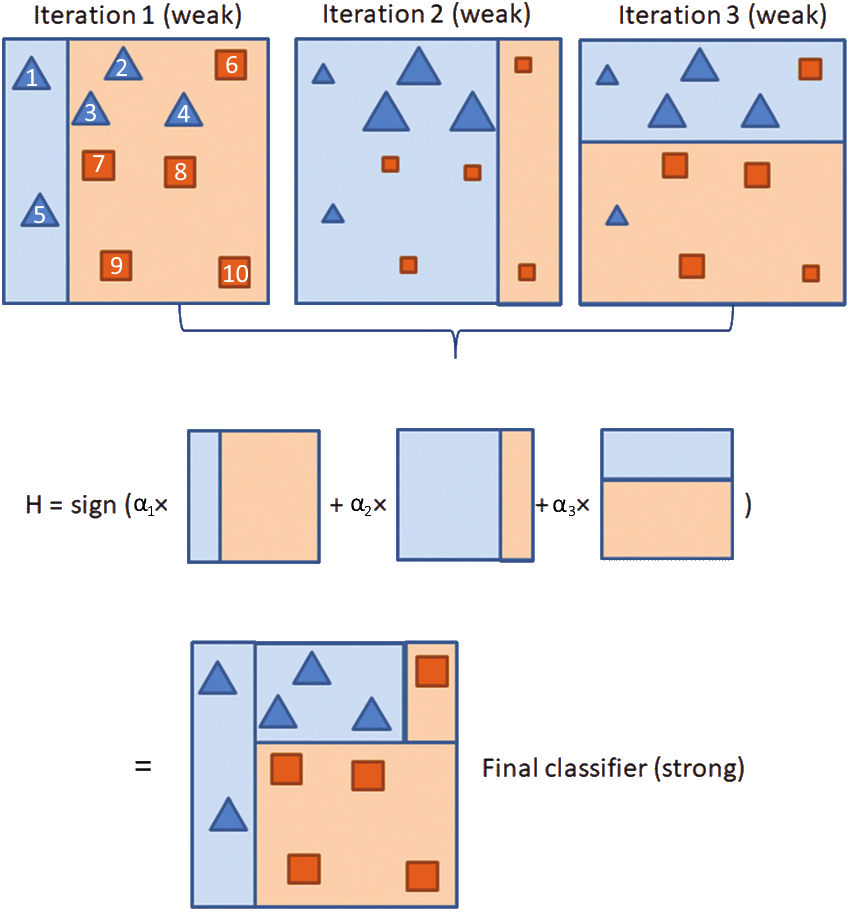
\includegraphics[width=\linewidth]{Images/adaBoostSchemaatic.png}
    \caption[Schematische Darstellung des AdaBoost-Prozesses]{Schematische Darstellung des AdaBoost-Prozesses. Blaue Dreiecke und orange Quadrate repräsentieren die Datenpunkte der beiden Klassen. (Quelle: ResearchGate, Alex Henderson et al.)}
    \label{fig:adaboost_schematic}
\end{figure}
  